% !TEX root = ../thesis.tex

\chapter{Auswertung}
\label{ch:auswertung}

In diesem Teil der Arbeit werden die Ergebnisse der Pipeline anhand von Referenzdaten validiert und bewertet.
Nach der Evaluation in \ref{sec:auswertung-daten} werden mögliche Fehlerquellen in \ref{sec:auswertung-fehler} genannt.
In \ref{sec:auswertung-zukunft} folgt ein Ausblick auf denkbare Erweiterungen in der Zukunft.



\section{Evaluation der Daten}
\label{sec:auswertung-daten}

Zur Evaluation der Pipeline wurden verschiedene Teile rekonstruiert und die Ergebnisse mit vorhandenen CAD-Modellen verglichen.
Zunächst wurden mit einer Kamera am Roboterarm bereits registrierte Punktwolken aufgenommen und zusammengeführt.
Anschließend wurden mit einer fest montierten Kamera mehrere Aufnahmen eines Teils gemacht, zwischen denen dieses leicht rotiert wurde.
Abschließend wurden mit der unbeweglichen Kamera jeweils zwei Aufnahmen einer Kiste gemacht, in der sich mehrere Teile gleicher Art befanden.
Im ersten Fall waren diese räumlich gut getrennt, im zweiten Fall handelte es sich um eine volle Kiste.

Da die generierte Rekonstruktion nicht am Referenzmodell ausgerichtet ist, wurde zum Vergleich eine manuelle Grobregistrierung durchgeführt.
Diese wurde anschließend durch eine lokale Registrierung durch ICP auf Basis der Vertices verfeinert.


\subsection{Werte}
\label{subsec:auswertung-daten-werte}

Als Qualitätsmetrik wurde die Cloud-Mesh-Distanz zwischen Rekonstruktion und Ground Truth gewählt.
Dabei wird die durchschnittliche Distanz zwischen Vertices und den nächsten Faces des Vergleichobjekts betrachtet.

\begin{table}[H]
	\centering
	\begin{tabular}{| c || c | c | c | c |}
		\hline
		\textbf{Distanzen [mm]} & Rad & Zahnrad & Gehäuse & T-Stücke\\
		\hline\hline
		Fix & $0.855$ & $0.462$ & $0.364$ & $0.486$\\
		\hline
		Rotation & $0.921$ & $0.558$ & $0.751$ & $0.333$\\
		\hline
		Seg. 1 \ac{ECE} & $0.527$ & $0.318$ & $0.238$ & $0.294$\\
		\hline
		Seg. 1 \ac{RG} & $0.842$ & $0.331$ & $0.819$ & $0.316$\\
		\hline
		Seg. 1 Watershed & $0.586$ & $0.315$ & $0.756$ & $0.305$\\
		\hline
		Seg. 2 \ac{ECE} & $1.322$ & $0.393$ & $0.549$ & $0.488$\\
		\hline
		Seg. 2 \ac{RG} & $1.089$ & $0.383$ & $0.491$ & $0.326$\\
		\hline
		Seg. 2 Watershed & $0.703$ & $0.411$ & $0.701$ & $0.297$\\
		\hline
	\end{tabular}
	\caption{Cloud-Mesh-Distanzen von Rekonstruktion zu Ground Truth}
	\label{tab:dist-mesh-gt}
\end{table}

In \autoref{tab:dist-mesh-gt} sind die Distanzen von den Vertices der Rekonstruktion zu den Faces des Referenzmodells zu sehen.
Diese können als Qualitätsmaß für die Regionen angesehen werden, in denen eine Oberfläche rekonstruiert wurde.

Bei Betrachtung der Werte fällt auf, dass die Segmentierung mit \ac{ECE} bei räumlich getrennten Objekten für alle getesteten Teile die geringste Distanz liefert.
Weiterhin kann beobachtet werden, dass \ac{ECE} bei geringer räumlicher Entfernung häufig zu einer höheren Distanz führt.

Die Segmentierung führt im Fall einer vollen Kiste außerdem je nach Objekt zu einer Verringerung oder Erhöhung der Distanz.
\ac{ECE} liefert beispielsweise für das Einkaufswagenrad sehr hohe Werte, während beim Zahnrad geringere Entfernungen als die Rekonstruktion über die mobile Kamera erzielt werden können.
Bei Wahl der Watershed-Segmentierung sind die Distanzen beim Rad jedoch deutlich niedriger.

\begin{table}[H]
	\centering
	\begin{tabular}{| c || c | c | c | c |}
		\hline
		\textbf{Distanzen [mm]} & Rad & Zahnrad & Gehäuse & T-Stücke\\
		\hline\hline
		Fix & $10.414$ & $2.468$ & $1.512$ & $2.398$\\
		\hline
		Rotation & $10.184$ & $2.513$ & $2.351$ & $3.224$\\
		\hline
		Seg. 1 \ac{ECE} & $11.097$ & $2.734$ & $2.692$ & $3.840$\\
		\hline
		Seg. 1 \ac{RG} & $18.414$ & $2.963$ & $5.831$ & $3.828$\\
		\hline
		Seg. 1 Watershed & $25.140$ & $7.005$ & $6.205$ & $4.449$\\
		\hline
		Seg. 2 \ac{ECE} & $19.703$ & $3.253$ & $7.711$ & $3.656$\\
		\hline
		Seg. 2 \ac{RG} & $19.744$ & $3.084$ & $4.675$ & $3.679$ \\
		\hline
		Seg. 2 Watershed & $16.056$ & $4.647$ & $3.536$ & $5.071$\\
		\hline
	\end{tabular}
	\caption{Cloud-Mesh-Distanzen von Ground Truth zu Rekonstruktion}
	\label{tab:dist-gt-mesh}
\end{table}

\autoref{tab:dist-gt-mesh} zeigt die Distanz von den Vertices des Referenzobjekts zu den Faces der Rekonstruktion.
Diese ist insbesondere in jenen Regionen sehr hoch, in denen Lücken in der Rekonstruktion vorhanden sind.

\begin{table}[H]
    \centering
    \begin{tabular}{| c || c | c | c | c |}
        \hline
        \textbf{Distanzverhältnis} & Rad & Zahnrad & Gehäuse & T-Stücke\\
        \hline\hline
        Fix & $0.08$ & $0.19$ & $0.24$ & $0.20$\\
        \hline
        Rotation & $0.09$ & $0.22$ & $0.32$ & $0.10$\\
        \hline
        Seg. 1 \ac{ECE} & $0.05$ & $0.12$ & $0.09$ & $0.08$\\
        \hline
        Seg. 1 \ac{RG} & $0.05$ & $0.11$ & $0.14$ & $0.08$\\
        \hline
        Seg. 1 Watershed & $0.02$ & $0.04$ & $0.12$ & $0.07$\\
        \hline
        Seg. 2 \ac{ECE} & $0.07$ & $0.12$ & $0.07$ & $0.13$\\
        \hline
        Seg. 2 \ac{RG} & $0.06$ & $0.12$ & $0.11$ & $0.09$\\
        \hline
        Seg. 2 Watershed & $0.04$ & $0.09$ & $0.20$ & $0.06$\\
        \hline
    \end{tabular}
    \caption{Verhältnis der Distanzen in \autoref{tab:dist-mesh-gt} und \autoref{tab:dist-gt-mesh}}
    \label{tab:dist-verhältnis}
\end{table}

Das Verhältnis der beiden Distanzmetriken ist in \autoref{tab:dist-verhältnis} und \autoref{fig:dist-verhältnis} sichtbar.
Im optimalen Fall, also einer vollständigen Rekonstruktion mit perfekter Qualität, konvergiert dieses Verhältnis gegen $1$, da dann die Distanz in beide Richtungen etwa gleich ist.
Ein höherer Wert steht hier also für eine höhere Vollständigkeit des rekonstruierten Meshs.

Aus den Werten erschließt sich, dass in den meisten Testfällen die Rotation das Mesh mit der höchsten Vollständigkeit geliefert hat.
Der Watershed-Algorithmus konnte im Vergleich mit den anderen Tests bei geringer räumlicher Distanz zwischen den Objekten nur den geringsten Teil der Oberfläche herstellen.

%\begin{figure}[H]
%	\centering
%	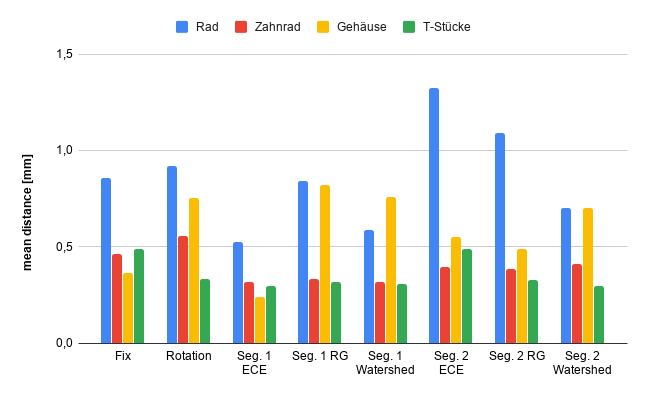
\includegraphics[width=0.49\textwidth]{images/segmentation/meanDistance1.png}
%	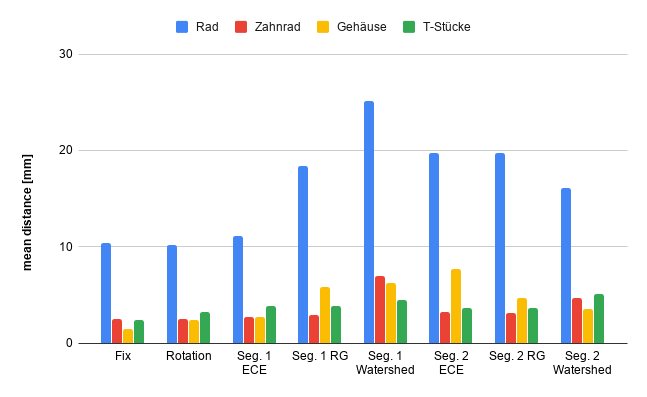
\includegraphics[width=0.49\textwidth]{images/segmentation/meanDistance2.png}
%	\caption{Diagramme der Werte in \autoref{tab:dist-mesh-gt} und \autoref{tab:dist-gt-mesh}}
%\end{figure}
\begin{figure}[H]
    \centering
    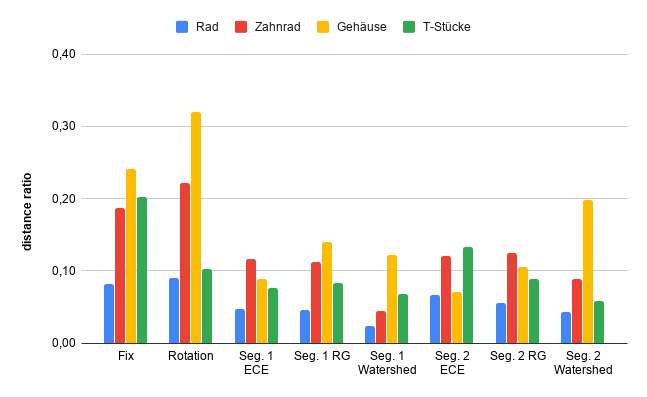
\includegraphics[width=0.75\textwidth]{images/segmentation/ratio.png}
    \caption{Diagramm der Distanzverhältnisse in \autoref{tab:dist-verhältnis}}
    \label{fig:dist-verhältnis}
\end{figure}


\subsection{Bewertung}
\label{subsec:auswertung-daten-bewertung}

Es zeigte sich, dass die Distanz von Rekonstruktion zu Ground Truth sich je nach Objekt bei unterschiedlichen Segmentierungen erhöht bzw. verringert.
Dies lässt darauf schließen, dass die Wahl der Segmentierungsmethode einen erheblichen Einfluss auf die Qualität der Rekonstruktion hat.
Jedoch gibt es offensichtlich nicht einen optimalen Ansatz, der in allen Fällen die besten Ergebnisse liefert.

Weiterhin wurde klar, dass die Rekonstruktion über Rotation eines einzelnen Objekts in den meisten Fällen die höchste Vollständigkeit liefert.
Dies lässt auf schlechte Ergebnisse bei der Segmentierung schließen, da die Objekte hier aus deutlich mehr Perspektiven zu sehen sein müssten.

Für die schlechten Ergebnisse bei der Segmentierung gibt es verschiedene Erklärungen.
Ist die Szene untersegmentiert, also nicht zusammengehörende Objekte noch in einem Cluster, kann das entsprechende Segment nicht integriert werden.
Die Information der darin enthaltenen Objekte gehen somit verloren.
Ein anderer Fall ist die Übersegmentierung der Szene.
Hier kann es vorkommen, dass nur wenige Punkte in einem Cluster enthalten sind und die Registierung des Objekts somit schwierig ist.
Unter Umständen kann keine eindeutige Position gefunden werden und somit gehen wieder wertvolle Informationen verloren.



\section{Fehlerbetrachtung}
\label{sec:auswertung-fehler}

Bei Aufnahme der Testdatensätze können mögliche Fehler entstanden sein, die das Ergebnis der Evaluation verfälschen.
Die folgende Liste stellt einen Auszug verschiedener Fehlerquellen dar.

\begin{itemize}
    \item unvermeidbares Sensorrauschen
    \item Spiegelungen durch einfallendes Sonnenlicht
    \item Ground Truth CAD-Modelle passen nicht zu tatsächlich vorhandenen Objekten
    \item tatsächlich vorhandene Objekte sind nicht exakt gleich
    \item unbeabsichtigte Bewegung des Objekts bei Rekonstruktion über Roboter
    \item fehlerhafte Ausrichtung zwischen generiertem Mesh und Referenz
\end{itemize}



\section{Zukünftige Arbeit}
\label{sec:auswertung-zukunft}

In der \nameref{subsec:auswertung-daten-bewertung} hat sich gezeigt, dass die Qualität des rekonstruierten Meshs abhängig vom Erfolg der Segmentierung ist.
Hier ließe sich eine deutliche Verbesserung erzielen, indem intelligentere Verfahren eingesetzt würden.
Eine Option wäre ein künstliches neuronales Netz, welches speziell auf industrielle Bauteile trainiert ist.

Eine andere Erweiterungsmöglichkeit bietet die Triangulation.
Hier könnten die Verschattungen der Objekte genutzt werden, um die Qualität der Rekonstruktion zu verbessern.
Diesen Ansatz verfolgen beispielsweise auch \citeauthor{kazhdan2020poisson} in \cite{kazhdan2020poisson}.

Weiterhin wäre es eine Möglichkeit, Informationen durch Nutzereingaben zu erlangen.
Dies könnte sowohl den Bereich der Segmentierung als auch der Registrierung umfassen.

Im Moment können Symmetrien und Spiegelungen in den Objekten nur sehr eingeschränkt betrachtet werden.
Würden diese berücksichtigt, könnte ein deutlich vollständigeres Mesh generiert werden.


